%!TEX program = lualatex
\documentclass[aspectratio=169]{beamer}
\usepackage[absolute]{textpos}
\usepackage{multirow}
\usepackage{tabto}
\usepackage{adjustbox}
\usepackage{enumitem}
\usepackage{setspace}
\usepackage{soul}
\usepackage{fancyvrb}

\usepackage{tikz}
\usetikzlibrary{arrows,shapes}
\tikzstyle{every picture}+=[remember picture]
\tikzstyle{na} = [baseline=-.5ex]

\usetheme{BMCV}

\title{Computermethoden: Computer Vision\\Part 6: Python Programming}
%\subtitle{} % if needed
\author{Leonid Kostrykin \and Karl Rohr}
\institute[BMCV Group, Heidelberg University and DKFZ]{Biomedical Computer Vision Group (BMCV) \\ BioQuant, IPMB, Heidelberg University}
\date{}

\usepackage{pythonhighlight}
\usepackage{keystroke}

\lstset{
  basicstyle=\ttfamily\scriptsize,
  keepspaces=true,
  backgroundcolor=\color{white},
  basewidth=0.5em,
  escapeinside=||
}

\newenvironment{commonmistake}[1]{\begin{minipage}{#1}%
  \setbeamercolor{block body}{bg=red!10,fg=black}
  \setbeamercolor{block title}{bg=red,fg=white}
  \begin{block}{Common mistake}}{\end{block}\end{minipage}}

%%% Comment out if needed:
%% Place an Outline Slide after each new section (not section*):
%\AtBeginSection[]%
%{%
%	\begin{frame}[plain,noframenumbering]{Outline}
%		\tableofcontents[currentsection]
%	\end{frame}
%}

\newcommand\makesectionframe[1]{%
    \begin{frame}[noframenumbering]{}%
        \begin{beamercolorbox}{title}%
        \centering\usebeamerfont{title} #1%
        \end{beamercolorbox}%
    \end{frame}}

\newcommand\undefined{\textit{\textcolor{black!50}{undefined}}}

\newcommand\indentationhint{\makebox{\textbf{Indentation:} \alert{\underline{4$\times$ whitespace!} (or \Tab)}}}

\newcommand\hilite[1]{{\setlength{\fboxrule}{2pt}\adjustbox{bgcolor=yellow, cframe=yellow {\fboxrule} {\fboxsep} -\fboxrule-\fboxsep}{#1}}}

\def\hiliteon<#1>#2{\alt<#1>{\hilite{#2}}{#2}}

\newcommand\whitebox[1]{\setlength{\fboxrule}{3pt}{\adjustbox{bgcolor=white, cframe=white {\fboxrule} {\fboxsep} -\fboxrule-\fboxsep}{\parbox{\linewidth + 2 \fboxsep}{#1}}}}


\begin{document}
\begin{frame}[title,noframenumbering]
\titlepage%
\end{frame}


\begin{frame}{Contents}
\alert{Introduction to Python programming:}
\begin{itemize}
\item Python resources
\item Characteristics of Python
\item Basic elements: Data types, variables, operators
\item Control structures: Selection, iteration
\item Re-usable code: Functions, modules
\item Data structures: Lists, multi-dimensional arrays
\item Understanding errors \& common mistakes
\end{itemize}
\end{frame}


\begin{frame}{Python resources}
    \begin{columns}[onlytextwidth]
    \column{0.75\textwidth}
    \alert{Official Python 3 tutorial:}
    \begin{itemize}
        \item \url{https://docs.python.org/3/tutorial/}
    \end{itemize}
    \column{0.25\textwidth}
    \begin{flushright}
    
\includegraphics[trim=145pt 170pt 180pt 145pt,clip,width=\linewidth]{Logos/python.png}
    \end{flushright}
    \end{columns}
    \vskip2ex
    \alert{Python 3 course on codecademy:}
    \begin{itemize}
        \item \url{https://www.codecademy.com/learn/learn-python-3}
        \item Paid subscription required, but free for 7 days
    \end{itemize}
    \vskip2ex
    \whitebox{\begin{columns}[onlytextwidth]
    \column{0.75\textwidth}
    \alert{Further resources:}
    \begin{itemize}
        \item \url{https://jupyter.org} -- IDE for data analysis
        \item \url{https://www.anaconda.com} -- Recommended software for installing/managing Python and additional modules
    \end{itemize}
    \column{0.25\textwidth}
    \begin{flushright}
    
\includegraphics[width=0.8\linewidth]{Logos/jupyter.pdf}\\\vskip 1.5ex%
    
\includegraphics[width=0.8\linewidth]{Logos/conda.png}%
    \end{flushright}
    \end{columns}}
\end{frame}


%\makesectionframe{Characteristics of Python}


\begin{frame}{Python in 2019}
    \begin{columns}
    \column{.46\textwidth}
    \whitebox{\begin{itemize}
        \item Python was created by \alert{Guido van Rossum} and first released in 1991
        \item Python 2 was released in 2000 and will be discontinued in 2020
        \item \alert{Python Software Foundation} launched 2001, is a nonprofit organization devoted to continued development of the Python programming language
        \item Python 3 was first released in 2008
        \item \textbf{Freely available!}
    \end{itemize}}
    \column{.54\textwidth}
    
\includegraphics[width=\textwidth]{Images/jaxenter20190410.png}
    \scriptsize\resizebox{\linewidth}{!}{\url{https://jaxenter.com/stack-overflow-dev-survey-2019-157815.html}}
    \end{columns}
\end{frame}


\begin{frame}{Characteristics of Python}
    \alert{High-level general-purpose programming language}
    \begin{itemize}
        \item Interpreted, dynamically typed, garbage-collected
        \item Very easy to write and understand
        \begin{itemize}
            \item English keywords
            \item Object-oriented and duck-typed
        \end{itemize}
        \item Well-suited for image and data analysis
        \item Widely used in scientific computing
    \end{itemize}
\end{frame}


\begin{frame}{Python: Object-oriented and duck-typed}
    Python is \alert{object-oriented}. What does this mean?
    \begin{itemize}
        \item Python programs consist of \alert{objects} which
        \begin{itemize}
            \item perform certain tasks
            \item interact with each other
        \end{itemize}
        \item An \alert{object} comprises \alert{attributes} (data) and \alert{methods} (behaviours)
    \end{itemize}
    \begin{textblock*}{4cm}(120mm,8mm) % {block width} (coords)
        \scalebox{-1}[1]{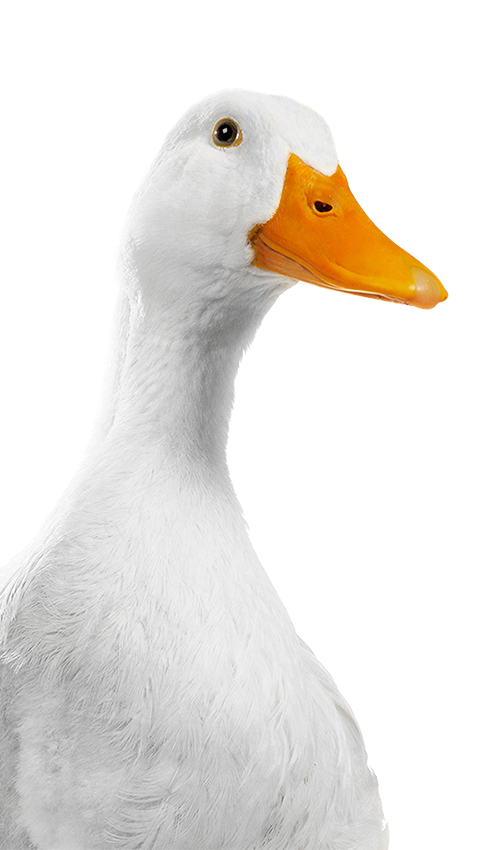
\includegraphics[width=4cm]{Images/duck.png}}
    \end{textblock*}
    \begin{block}{Python is duck-typed}
    \begin{quote}
        Duck typing in computer programming is an application of the \alert{duck test} -- \textbf{``If it walks like a duck and it quacks like a duck, then it must be a duck''} -- to determine if an object can be used for a particular purpose.
    \end{quote}
    \footnotesize{-- \url{https://en.wikipedia.org/wiki/Duck_typing}}
    \end{block}
    \vspace{3pt}
\end{frame}


\begin{frame}{Objects and types}
    \begin{itemize}
        \item An object (e.g., ``Donald'') is instantiated (created) from a \alert{type} (e.g., ``Duck'')
        \item An object's \alert{type} defines
        \begin{itemize}
            \item \textbf{which} methods the \textbf{object} offers (e.g., walking, quaking, \ldots)
            \item \textbf{which} attributes the \textbf{object} possesses (e.g., age, color, \ldots)
            \item \alert{\ldots but not their values!} (e.g., Donald has a \emph{different} age and color than Daisy)
        \end{itemize}
    \end{itemize}
\end{frame}


\begin{frame}{Python Programming}
    \begin{columns}[T,onlytextwidth]
    \column{.7\linewidth}
    \alert{Input-process-output (IPO)} \textbf{model of a program}
    \begin{enumerate}
        \item Loads input data (e.g., an image)
        \item Processes the loaded data
        \item Outputs the processed data (e.g., analysis results)
    \end{enumerate}
    \column{.3\linewidth}
    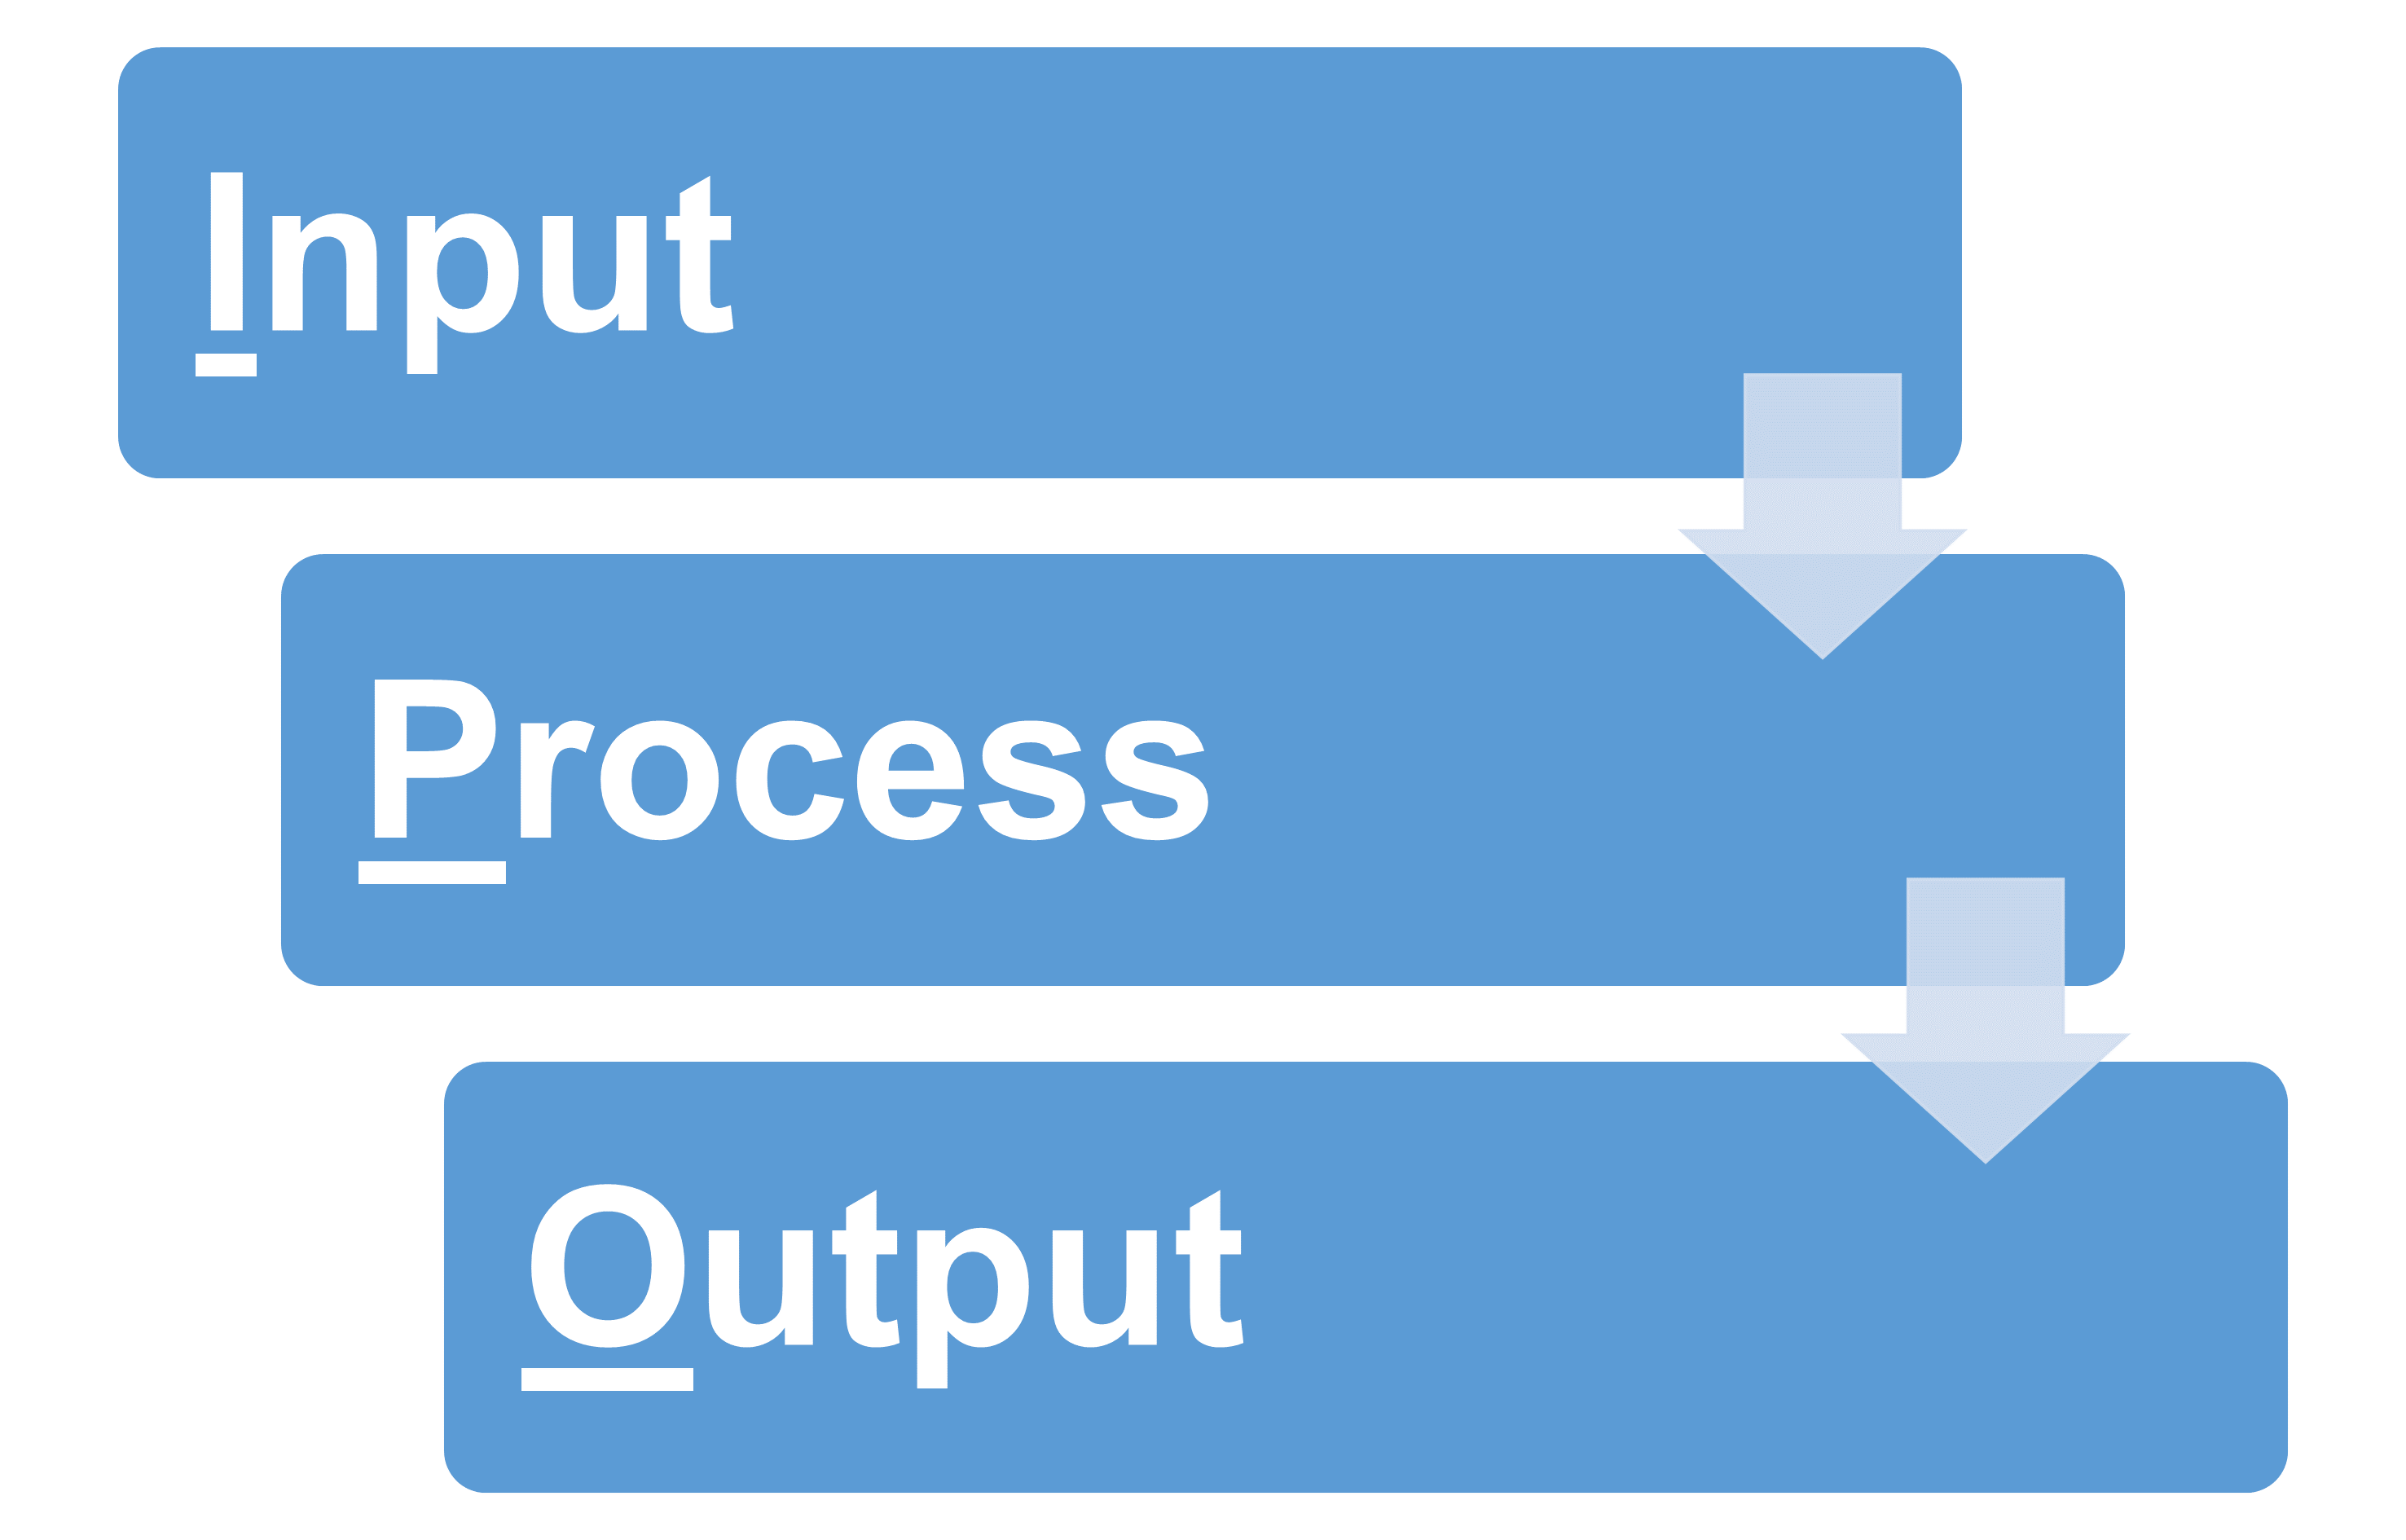
\includegraphics[width=\linewidth]{Images/ipo.png}
    \end{columns}
    \vskip2ex
    \whitebox{\alert{Cycle of Python programming steps}
    \begin{enumerate}
        \item Write Python code
        \item Run the written Python code
        \item Compare the output results with the expected results
        \item If something is wrong: \quad\alert{(this is the \underline{usual} case!)}\\
            Critically re-consider your code \rightarrow\ Fix errors \rightarrow\ Return to step 2
    \end{enumerate}}
\end{frame}


\begin{frame}[fragile]{A simple Python program}
\begin{python}
print('Welcome to Python programming!')
\end{python}
    \begin{itemize}
        \item \pyth{print} is a \alert{built-in function}
        \item Prints \emph{one line of text} to the \alert{standard output} (e.g., the screen)
        \item The part between ``\pyth{(}'' and ``\pyth{)}'' are the \textbf{function parameters}
        \begin{itemize}
            \item For \pyth{print}, this is the \textbf{content to be printed}
            \item Here a \alert{string} (text, must be put in quotes like ``\pyth{'}\ldots\pyth{'}'') is printed
        \end{itemize}
        \item In strings, special characters can be inserted:
        \begin{center}\begin{tabular}{llcll}
            \texttt{\string\\} & backslash character & & \texttt{\string\t} & tab stop \\
            \texttt{\string\n} & line break & & \texttt{\string\'} & single quote
        \end{tabular}\end{center}
    \end{itemize}
\end{frame}


\makesectionframe{Data types, variables, and operators}


\begin{frame}[fragile]{Variables, assignments, and expressions}
\alert{Assignment syntax}
\begin{python}
variable = value
\end{python}
\vskip2ex
\alert{Assigns \pyth{value} to \pyth{variable}, where \pyth{value} can be}
\begin{itemize}
    \item An \textbf{object} (e.g., number, string, list, duck, \ldots)
    \item An \textbf{expression} which \emph{evaluates} to an object \\(e.g., the expression ``\pyth{6 + 5}'' evaluates to the numeric object \pyth{11})
\end{itemize}
The \pyth{variable} then \textbf{represents} the object which it was assigned
\vskip2ex
\alert{Combined expressions:} The expression ``\pyth{3 * (6 + 5)}'' evaluates to \pyth{33}
\end{frame}


\begin{frame}[fragile]{Numbers, strings, and variables}
\begin{columns}[T]
\column{.5\textwidth}
\begin{python}
var1 = 2
var2 = 11
var3 = var1 + var2
print(var3)
var1 = var3
print(var1 * 2 + 0.5)
\end{python}
\vskip2ex
\alert{Output}
\begin{verbatim}
13
26.5
\end{verbatim}
\column{.5\textwidth}
\begin{python}
var1 = '42'
var2 = 'What is the answer?'
var3 = var2 + ' ' + var1
print(var3)
\end{python}
\textbf{Reminder:} String-type objects \emph{start and end} with single quotes!
\vskip2ex
\alert{Output}
\begin{verbatim}
What is the answer? 42
\end{verbatim}
\end{columns}
\vskip2ex
\begin{center}
    \visible<2>{\hilite{\textbf{$\Rightarrow$} The \alert{behaviour} of the ``\pyth{+}'' operator depends on the \alert{type} of the operands!}}
\end{center}
\end{frame}


\begin{frame}{Built-in types}
    In Python, \alert{numbers} are represented by \underline{one of two types}
    \begin{itemize}
        \item An object of type \pyth{float} can be \alert{any decimal number} between $\pm 1.8 \cdot 10^{308}$ \\ but \textbf{most numbers cannot be represented \underline{exactly}} (limited machine precision)
        \item An object of type \pyth{int} can be \alert{any integer number} (e.g., \texttt{-123}, \texttt{0}, \texttt{321}, \ldots)
    \end{itemize}
    \vskip3ex
    \begin{columns}[t,onlytextwidth]
    \column{.55\textwidth}
    \alert{Examples for objects of type \pyth{float}} \\
    \texttt{-123.2}\textbf,\enspace\texttt{1.2e3}\textbf,\enspace \texttt{0.0}\textbf,\enspace\texttt{12.0}\textbf,\enspace\texttt{3.14}\textbf,\enspace\ldots
    \column{.45\textwidth}
    \alert{Examples for objects of type \pyth{int}} \\
    \texttt{-123}\textbf,\enspace\texttt{0}\textbf,\enspace\texttt{321}\textbf,\enspace\ldots
    \end{columns}
    \vskip4ex
    \alert{Many other types:} \texttt{str}, \texttt{list}, \texttt{dict}, \texttt{set}, \texttt{frozenset}, \texttt{complex}, \texttt{bool}, \ldots
\end{frame}


\begin{frame}{Operators and types}
    Different \alert{operations} (behaviours) performed by different \alert{operators} and \alert{types}:
    \begin{center}
    \resizebox{\textwidth}{!}{\begin{tabular}{l||c|c|c}
         \multirow{2}{20mm}{\alert{Pythonic expression}} & \pyth{op1} and \pyth{op2} are \alert{numbers} & \multicolumn{2}{c}{\pyth{op1} is a \alert{list} or \alert{string} and \pyth{op2} is\ldots} \\ \cline{2-4}
         & (e.g., \textbf{\pyth{float}} or \textbf{\pyth{int}}) & an \textbf{\pyth{int}} & \alert{same type} as \pyth{op1} \\ \hline\hline
         \pyth{op1 + op2} & \textbf{sum} of \pyth{op1} and \pyth{op2} & \undefined & \textbf{concatenation} of \pyth{op1} and \pyth{op2} \\ \hline
         \pyth{op1 - op2} & \textbf{difference} of \pyth{op1} and \pyth{op2} & \multicolumn{2}{c}{\undefined} \\ \hline
         \pyth{op1 * op2} & \textbf{product} of \pyth{op1} and \pyth{op2} & \pyth{op1} \textbf{repeated} \pyth{op2} times & \undefined \\ \hline
         \pyth{op1 / op2} & (true) \textbf{division} of \pyth{op1} and \pyth{op2} & \multicolumn{2}{c}{\undefined} \\ \hline
         \pyth{op1 \%}\texttt{ }\pyth{op2} & \textbf{modulo} of \pyth{op1} and \pyth{op2} & \multicolumn{2}{c}{\undefined} \\ \hline
         \pyth{op1 //}\texttt{ }\pyth{op2} & \textbf{integer division} of \pyth{op1} and \pyth{op2} & \multicolumn{2}{c}{\undefined}
    \end{tabular}}
    \end{center}
    \vskip1ex
    \alert{Note:} ``\pyth{op1 +=}\texttt{ }\pyth{op2}'' is a shorthand for ``\pyth{op1 = op1 + op2}''. The same holds analogously for the other operators (\pyth{-=}, \pyth{*=}, \pyth{/=}, \pyth{\%=}, \pyth{//=}).
\end{frame}


\begin{frame}{True division vs integer division}
    \label{frame:true_division_vs_integer_division}
    \def\tmpitemsep{0.2em}
    \begin{columns}[t,onlytextwidth]
    \column{.45\textwidth}
    \alert{True division}
    \begin{itemize}
        \setlength\itemsep{\tmpitemsep}
        \item ``\pyth{6 /}\texttt{ }\pyth{3}'' yields ``\pyth{2.0}'' (\pyth{float})
        \item ``\pyth{7 /}\texttt{ }\pyth{4}'' yields ``\pyth{1.75}'' (\pyth{float})
        \item ``\pyth{17 /}\texttt{ }\pyth{5}'' yields ``\pyth{3.4}'' (\pyth{float})
    \end{itemize}
    \column{.55\textwidth}
    \alert{Integer division:} Fractal part truncated
    \begin{itemize}
        \setlength\itemsep{\tmpitemsep}
        \item ``\pyth{6 //}\texttt{ }\pyth{3}'' yields ``\pyth{2}'' (\pyth{int})
        \item ``\pyth{7 //}\texttt{ }\pyth{4}'' yields ``\pyth{1}'' (\pyth{int})
        \item ``\pyth{17 //}\texttt{ }\pyth{5}'' yields ``\pyth{3}'' (\pyth{int})
    \end{itemize}
    \end{columns}
    \vskip2ex
    \whitebox{\alert{Modulo operator:} Remainder after integer division (fractal part nominator)
    \begin{itemize}
        \setlength\itemsep{\tmpitemsep}
        \item ``\pyth{6 \%}\texttt{ }\pyth{3}'' yields ``\pyth{0}'' (\pyth{int}, fractal part: $0/4=0$)
        \item ``\pyth{7 \%}\texttt{ }\pyth{4}'' yields ``\pyth{3}'' (\pyth{int}, fractal part: $3/4=0.75$)
        \item ``\pyth{17 \%}\texttt{ }\pyth{5}'' yields ``\pyth{2}'' (\pyth{int}, fractal part: $2/5=0.4$)
        \item \textbf{Question:} \textit{Is ``\pyth{op1 //}\texttt{ }\pyth{op2}'' a shorthand for ``\pyth{(op1 - op1 \%}\texttt{ }\pyth{op2)} \pyth{/ op2}''?}
        \item \textbf{Application example:} \textit{Determine whether one number is a multiple of the other}
    \end{itemize}}
\end{frame}


\begin{frame}{Other mathematical operators}
    \textbf{Remember:} \alert{The operators \pyth{+}, \pyth{-}, \pyth{*}, \pyth{\%}, \pyth{//}} yield an object of type \pyth{int} if \pyth{op1} and \pyth{op2} both are of type \pyth{int}, and \pyth{float} otherwise
    \vskip1ex
    \begin{columns}[T,onlytextwidth]
    \column{.4\textwidth}
    \alert{Examples}
    \begin{itemize}
        \item ``\pyth{6 +}\texttt{ }\pyth{2}'' yields ``\pyth{8}'' (\pyth{int})
        \item ``\pyth{6 +}\texttt{ }\pyth{2.0}'' yields ``\pyth{8.0}'' (\pyth{float})
    \end{itemize}
    \column{.6\textwidth}
    \resizebox{\textwidth}{!}{\begin{tabular}{l||c|c}
         \multirow{2}{20mm}{\alert{Pythonic expression}} & \multicolumn{2}{c}{\alert{Type of the result}} \\ \cline{2-3} & \pyth{op1} \textbf{or} \pyth{op2} is \pyth{float} & \pyth{op1} \textbf{and} \pyth{op2} are \pyth{int} \\ \hline\hline
         \pyth{op1 + op2} & \pyth{float} & \pyth{int} \\ \hline
         \pyth{op1 - op2} & \pyth{float} & \pyth{int} \\ \hline
         \pyth{op1 * op2} & \pyth{float} & \pyth{int} \\ \hline
         \pyth{op1 / op2} & \pyth{float} & \pyth{float} \\ \hline
         \pyth{op1 \%}\texttt{ }\pyth{op2} & \pyth{float} & \pyth{int} \\ \hline
         \pyth{op1 //}\texttt{ }\pyth{op2} & \pyth{float} & \pyth{int}
    \end{tabular}}
    \end{columns}
    \vskip2ex
    \whitebox{\alert{Why is this important?} \\
    \textbf{Example:} Indexing -- \emph{see later, be patient!}}
\end{frame}


\begin{frame}[t,fragile]{String formatting}
\vskip2ex
\begin{python}
day   = 31
month = 'January'
year  = 2019
\end{python}
\alert{Task:} Print the above variables in a canonical date format (``\texttt{31. January 2019}'')
\vskip1ex

\begin{onlyenv}<1-2>{\textbf{Is this a correct solution?}}
\begin{python}
print(day + '. ' + month + ' ' + year)
\end{python}
\visible<2>{\alert{It is wrong!} The ``\pyth{+}''-operators are used for operands of \emph{different} types (\textbf{numbers} and \textbf{strings}). This case is \emph{undefined!}}
\end{onlyenv}

\begin{onlyenv}<3>{\textbf{Correct solutions:}}
\begin{python}
print(str(day) + '. ' + str(month) + ' ' + str(year))
\end{python}
\begin{columns}[T,onlytextwidth]
\column{.38\linewidth}
\begin{python}
print(f'{day}. {month} {year}')
\end{python}
\column{.56\linewidth}
\vspace{-7pt}
\parbox{\linewidth+1cm}{\begin{itemize}[leftmargin=0mm]\setlength\itemsep{0em}
    \item \small ``\textbf{\pyth{f}}''-prefix creates a \alert{formatted string}
    \item \small Substitutes ``\pyth{\{day\}}'' by the value of the variable ``\pyth{day}'', \ldots
\end{itemize}}
\end{columns}
\vspace{3mm}
\begin{columns}[T,onlytextwidth]
\column{.45\linewidth}
\begin{python}
print('%d. %s %d' % (day, month, year))
\end{python}
\column{.5\linewidth}
\vspace{3pt}
\small C-style string formatting (old-fashioned)
\end{columns}
\end{onlyenv}
\end{frame}


\makesectionframe{Selections and iterations}


\begin{frame}[fragile]{Selections}
\centering\alert{Structures of the \pyth{if}-statement permitted in Python}
\begin{columns}
\column{.5\textwidth}
\begin{python}
if condition:
    instruction1
    instruction2
\end{python}
\begin{python}
if condition1:
    instruction1
    instruction2
else:
    instruction3
    instruction4
\end{python}
\indentationhint
\column{.5\textwidth}
\begin{python}
if condition1:
    instruction1
    instruction2
elif condition2:
    instruction3
    instruction4
else:
    instruction3
    instruction4
\end{python}
\begin{python}
if condition1: instruction1
elif condition2: instruction2
else: instruction3
\end{python}
\end{columns}
\end{frame}


\begin{frame}[fragile]{Conditions}
\alert{Conditions can be implemented as}
\begin{itemize}
\item An object of type \pyth{bool} (either of the two built-in objects ``\pyth{True}'' or ``\pyth{False}'')
\item A variable which \emph{represents} an object of type \pyth{bool} -- \alert{Example:}
\begin{python}
var1 = True
if var1: print('var1 is True')
\end{python}
\item An expression which \emph{evaluates} to an object of type \pyth{bool}\\(e.g., uses \emph{equality or relational operators}) -- \alert{Example:}
\begin{python}
var1 = True
if not var1: print('var1 is False')
\end{python}
\end{itemize}
\end{frame}


\begin{frame}{Equality or relational operators}
    Expressions which evaluate to an object of type \pyth{bool}:
    \begin{center}
    \resizebox{\textwidth}{!}{\begin{tabular}{l||l}
        \alert{Pythonic expression} & Evaluates to \pyth{True} if\ldots\ (and \pyth{False} otherwise) \\
        \hline\hline
        \multicolumn{2}{l}{\textit{Equality operators}} \\ \hline
        \pyth{op1 ==}\texttt{ }\pyth{op2} & \ldots\pyth{op1} is \textbf{equal} to \pyth{op2} \\ \hline
        \pyth{op1 !=}\texttt{ }\pyth{op2} & \ldots\pyth{op1} is \textbf{not equal} to \pyth{op2} (equivalent to ``\pyth{not op1 ==}\texttt{ }\pyth{op2}'') \\ \hline
        \multicolumn{2}{l}{\textit{Relational operators}} \\ \hline
        \pyth{op1 <}\texttt{ }\pyth{op2} & \ldots\pyth{op1} is \textbf{less} than \pyth{op2} \\ \hline
        \pyth{op1 >}\texttt{ }\pyth{op2} & \ldots\pyth{op1} is \textbf{greater} than \pyth{op2} \\ \hline
        \pyth{op1 <=}\texttt{ }\pyth{op2} & \ldots\pyth{op1} is \textbf{less equal than or equal} to \pyth{op2} \\ \hline
        \pyth{op1 >=}\texttt{ }\pyth{op2} & \ldots\pyth{op1} is \textbf{greater than or equal} to \pyth{op2} \\ \hline
        \pyth{op1 in op2} & \ldots\pyth{op2} \textbf{contains} \pyth{op1} (only defined if \pyth{op2} is a string, list, \ldots)
    \end{tabular}}
    \end{center}
\end{frame}


\begin{frame}[fragile]{Example for \texttt{if}-conditions}
\begin{columns}[onlytextwidth]
\column{.6\textwidth}
\begin{python}
student_grade = 25
s1 = 'Passed!'
s2 = 'Failed!'

student_grade *= 2

if student_grade >= 50: res = s1
else: res = s2

res = f"Grade={student_grade} ==> {res}"
print(res)
\end{python}
\column{.3\textwidth}
\begin{onlyenv}<2->\alert{Output}
\begin{verbatim}Grade=50 ==> Passed!\end{verbatim}\end{onlyenv}
\end{columns}
\end{frame}


\begin{frame}[fragile]{Iterations}
\begin{columns}[T]
\column{.65\textwidth}
\alert{Structures of the \pyth{while}-loop in Python}
\begin{python}
while condition:
    instruction1
    instruction2
    ...
\end{python}
\vskip3ex
\indentationhint
\column{.45\textwidth}
\alert{Example}
\begin{python}
i = 0
while i < 10:
    print(i)
    i += 1
\end{python}
\alert{Output}
\begin{verbatim}
0
1
2
...
9
\end{verbatim}
\end{columns}
\end{frame}


\begin{frame}[fragile]{The \texttt{for}-loop and iterables}
\begin{center}The \pyth{while}-loop from the previous slide can be formulated as follows
\end{center}
\vspace{-2mm}
\begin{columns}[T]
\column{.5\textwidth}
\alert{Structures of the \pyth{for}-loop in Python}
\begin{python}
for item in iterable:
    instruction1
    instruction2
    ...
\end{python}
\column{.5\textwidth}
\alert{Example}
\begin{python}
for i in range(0, 10):
    print(i)
\end{python}
\indentationhint
\end{columns}
\vskip1ex
\whitebox{An \alert{iterable} can be any \textbf{object which contains items}, for example:
\begin{itemize}
    \item A \textbf{range} of \pyth{int} objects, \pyth{range(a, b)} corresponds to the \\\underline{\emph{half-closed}} interval $\mathbb Z \cap [a, b)$. \alert{Note:} \textbf{\pyth{a} and \pyth{b} must be of type \pyth{int}!}
    \item A \textbf{list} (sequence of arbitrary objects), a \textbf{string} (sequence of characters), \ldots
    \item More examples will be learned during the \emph{\underline{practical lab sessions}!}
\end{itemize}}
\vspace{6mm}
\end{frame}


\begin{frame}[fragile]{More loop examples}
\begin{columns}[T]
\column{.5\textwidth}
\alert{Example 1}
\begin{python}
product = 2
while product <= 10_000:
    product *= 2
print(product)
\end{python}
\textbf{Hint:} ``\pyth{10_000}'' is a more easily human-readable notation for \pyth{10000}
\visible<2->{\par\vskip2ex\alert{Output:} \texttt{16384}}
\column{.5\textwidth}
\alert{Example 2}
\begin{python}
result = ''
for character in 'Hello World':
    result = character + result
print(result)
\end{python}
\visible<3->{\par\vskip2ex\alert{Output:} \texttt{dlroW olleH}}
\end{columns}
\end{frame}


\makesectionframe{Functions and modules}


{\setbeamercovered{transparent}\begin{frame}{Re-usable code}
    Python supports \alert{code re-usability} at \underline{different levels}:
    \begin{enumerate}
        \item<1> \textbf{Classes} (e.g., specify the \emph{blueprint} of a duck, i.e., its \emph{attributes} and how it \emph{behaves}, then synthesize as many ducks as you want)
        \item<1-2> \textbf{Functions} (e.g., specify a receipt for how to roast \st{a duck} tofu \emph{once}, then roast many \st{ducks} tofus on an assembly line)
        \item<1-2> \textbf{Modules:} Collections of classes + functions for specific tasks (e.g., load and use the \emph{duck processing toolkit} someone else wrote, or write your own one)
    \end{enumerate}
\end{frame}}


\begin{frame}{Functions}
    \alert{Built-in functions}
    \vskip1ex
    \whitebox{\begin{itemize}
        \item \pyth{abs(number)} \tabto{3cm}-- computes $\left|x\right|$ where $x$ is a \pyth{number}
        \item \pyth{int(number)} \tabto{3cm}-- truncates the fractal part of \pyth{number} (yields an \pyth{int} object)
        \item \pyth{len(iterable)} \tabto{3cm}-- counts items in \pyth{iterable} (e.g., characters in a string)
        \item \pyth{pow(a, b)} \tabto{3cm}-- computes $a^b$ for any numbers \pyth{a} and \pyth{b}
        \item \pyth{print(value)} \tabto{3cm}-- prints \pyth{value} to the standard output
        \item \pyth{range(a, b)} \tabto{3cm}-- yields an iterable for \pyth{int} objects in $[a,b) \cap \mathbb{Z}$
        \item \pyth{round(number)} \tabto{3cm}-- rounds \pyth{number} to the closest integer value (yields \pyth{int})
        \item \pyth{str(value)} \tabto{3cm}-- converts \pyth{value} (e.g., \pyth{float}, \pyth{int}) to a string
        \item \pyth{sum(iterable)} \tabto{3cm}-- yields sum of items in \pyth{iterable} (e.g., numbers in a list)
        \item \textit{and many others\ldots}
    \end{itemize}}
\end{frame}


\begin{frame}[fragile]{Writing functions}
\begin{center}Lets define a \alert{re-usable function} ``\pyth{reverse}'' which \textbf{reverses a string}
\end{center}
\begin{columns}[T]
\column{.5\textwidth}
\alert{Syntax for function definitions}
\begin{python}
def function(parameters):
    instruction1
    instruction2
    ...
\end{python}
\indentationhint
\column{.5\textwidth}
\alert{Example}
\begin{python}
def reverse(string):
    result = ''
    for character in string:
        result = character + result
    return result
\end{python}
\end{columns}
\vskip1ex
\whitebox{\begin{itemize}
    \item The \pyth{return} instruction determines the object, which the function evaluates to
    \item The \pyth{return} instruction terminates the execution of the function
    \item \makebox[\linewidth][l]{The function evaluates to the object \pyth{None} if no \pyth{return} instruction is encountered}
\end{itemize}}
\end{frame}


\begin{frame}[fragile]{Examples for self-written functions}
\begin{columns}[onlytextwidth]
\column{.6\textwidth}
\begin{python}
def reverse(string):
    result = ''
    for character in string:
        result = character + result
    return result

reverse('Hello World')
reverse(reverse('Hello World'))
\end{python}
\column{.3\textwidth}
\begin{visibleenv}<2->\alert{Output}
\begin{verbatim}dlroW olleH\end{verbatim}\end{visibleenv}
\begin{visibleenv}<3->\
\begin{verbatim}Hello World\end{verbatim}\end{visibleenv}
\end{columns}
\end{frame}


\begin{frame}{Modules}
    \begin{textblock*}{4cm}(122mm,13mm) % {block width} (coords)
        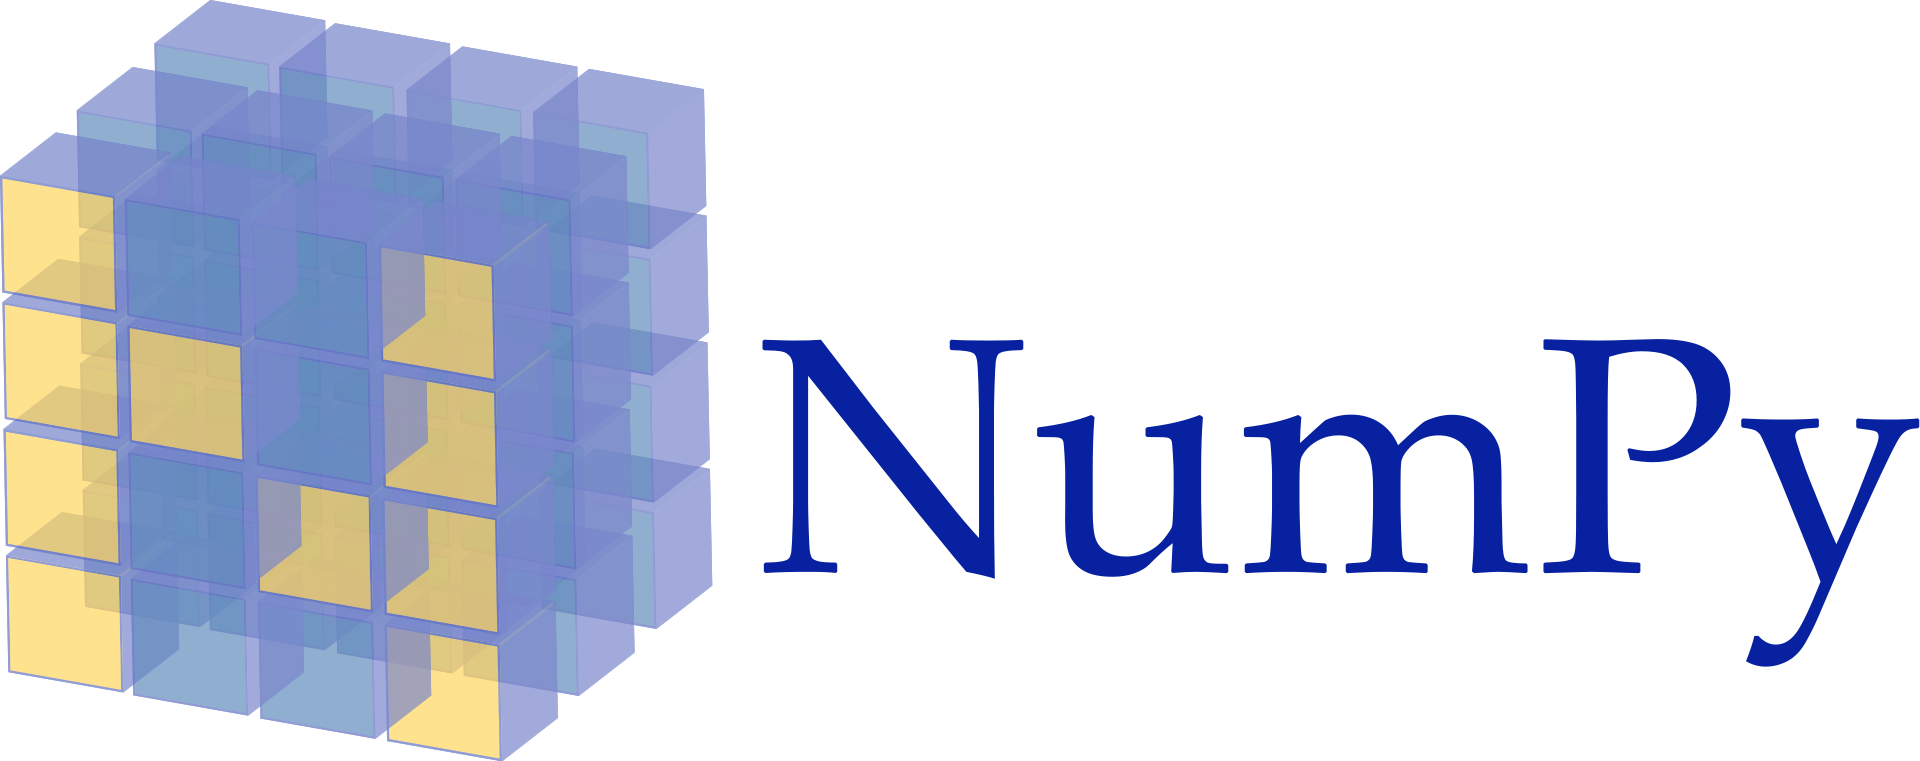
\includegraphics[height=1.5\baselineskip]{Logos/numpy.png}\\\vskip 0.6ex
        
\includegraphics[height=1.3\baselineskip]{Logos/scipy.png}\\\vskip 0.6ex
        
\includegraphics[height=1.3\baselineskip]{Logos/skimage.png}
    \end{textblock*}
    \textit{An ecosystem that can hardly be overlooked}
    \vskip3ex
    \alert{Popular low-level Python modules}
    \begin{itemize}
        \item \texttt{numpy} \tabto{20mm}-- numerical Python extensions  (linear algebra, \\\tabto{20mm}\phantom{-- }multi-dimensional arrays, \ldots)
        \item \texttt{scipy} \tabto{20mm}-- scientific computing (e.g., optimization, interpolation, \\\tabto{20mm}\phantom{-- }image processing, \dots)
    \end{itemize}
    \vskip2ex
    \alert{Popular high-level Python modules}
    \begin{itemize}
        \item \texttt{sklearn} \tabto{20mm}-- machine learning
        \item \texttt{skimage} \tabto{20mm}-- image processing (stand-alone + integrates into \texttt{sklearn})
    \end{itemize}
\end{frame}


\begin{frame}[fragile]{Loading and using modules}
\alert{Fundamentals of working with modules}
\begin{center}
\resizebox{\textwidth}{!}{\begin{tabular}{l|l|l}
    \alert{Purpose} & \alert{Syntax} & \alert{Example} \\
    \hline\hline
    \textbf{Loading} a module & \pyth{import module} & \pyth{import math} \\ \hline
    \textbf{Using an object} from a loaded module & \texttt{module.object} & \pyth{print(math.pi)} \\ \hline
    \textbf{Using a function} from a loaded module & \texttt{module.function(\ldots)} & \pyth{print(math.log10(10))}
\end{tabular}}
\end{center}
\vskip3ex
\alert{Hierarchical organization:} Some modules contain sub-modules -- \alert{Example:}
\begin{python}
import skimage.io
img = skimage.io.imread('filepath.tiff')
\end{python}
\whitebox{Reads the image from the file ``\texttt{filepath.tiff}'' as an object represented by \pyth{img}}
\end{frame}


\makesectionframe{Lists and multi-dimensional arrays}


\begin{frame}{Lists}
\begin{itemize}
\item \alert{So far:} A \textbf{single variable} \underline{represents} a \textbf{single object}
\begin{center}
\framebox{\texttt{variable}} $\xleftarrow{\text{assign}}$ \framebox{\texttt{object}}\,,\quad e.g.:\quad\pyth{var1 = 12}
\end{center}
\vskip3ex
\item \alert{A list} is an \textbf{object} which \underline{contains} \hiliteon<2->{references} to \textbf{multiple objects}
\begin{center}
\framebox{\texttt{list} (\texttt{object})} $\xleftarrow{\text{append}}$ \framebox{\texttt{object}}\,,\quad e.g.:\quad\begin{minipage}[t]{4cm}
\pyth{var1 = list()} \\
\pyth{var1.append(12)} \\
\pyth{var1.append(14)} \\
\pyth{var1.append(15)}
\end{minipage}
\end{center}\vskip1ex
\item<3> \textbf{Removing an object} from a list \underline{deletes the reference} (the object still exists) \\ \alert{Example:} \quad \begin{minipage}[t]{10cm}
\pyth{var1.remove(14)} \\
\pyth{print(var1)} \hspace{15mm} produces the output: \enspace\texttt{[12, 15]}
\end{minipage}
\end{itemize}
\end{frame}


\begin{frame}[fragile]{\texttt{list} indexing and iterating}
\label{frame:list_indexing_and_iterating}
\begin{columns}[T]
\column{0.21\linewidth}
\makebox[\linewidth][l]{\textbf{A list is a continuous sequence of object references} (\textit{``flat map of positions to objects''})}
\vspace{-2mm}\begin{python}
var1 = list()
var1.append(12)
var1.append(14)
var1.append(15)
var1.append(-3)
\end{python}
\column{0.18\linewidth}
\vspace{8mm}\resizebox{\textwidth}{!}{\begin{tabular}{c|c}
    \alert{Position} & \alert{Object} \\
    \hline\hline
    0 & \texttt{12} \\\hline
    1 & \texttt{14} \\\hline
    2 & \texttt{15} \\\hline
    3 & \texttt{-3} \\\hline
\end{tabular}}
\column{0.65\linewidth}
\vspace{8mm}\alert{Accessing data in a list}
\begin{itemize}
    \item \small\textbf{\pyth{len(var1)}}: Yields number of items in \pyth{var1}
    \item \small\textbf{\pyth{var1[i]}}: Represents the \pyth{i}-th item (entry) of the list (``\pyth{i}'' is called \emph{position} or \emph{index}) \\ \alert{Notes:} \hspace{-4pt}\begin{minipage}[t]{6cm}
        \vspace{-7pt}
        \begin{itemize}[noitemsep,topsep=0pt,nolistsep]
            \item \small \makebox{\hiliteon<2>{\pyth{i} must suffice $-\text{\pyth{len(var1)}} \leq \text{\pyth{i}} < \text{\pyth{len(var1)}}$}}
            \item \small \hiliteon<3>{\pyth{i=-1} refers to the last item}
            \item \small \hiliteon<3>{\pyth{i=-2} to the one before the last, \ldots}
            \item \small \hiliteon<4>{\pyth{i} must be an \pyth{int}}
        \end{itemize}
    \end{minipage}
\end{itemize}
\end{columns}
\vskip3ex
\begin{columns}[T]
\column{.45\linewidth}
\alert{Iteration by index}
\begin{python}
for i in range(0, len(var1)):
    print(var1[i])
\end{python}
\column{.3\linewidth}
\alert{Lists are iterable}
\begin{python}
for obj in var1:
    print(obj)
\end{python}
\column{.2\linewidth}
\alert{Output}
\footnotesize
\vspace{-2mm}\begin{verbatim}
12
14
15
-3
\end{verbatim}
\end{columns}
\end{frame}


\begin{frame}[fragile]{\texttt{list} indexing example}
\alert{Note:} \quad
\begin{minipage}[t]{28mm}%
\vspace{-3mm}\begin{python}
var1 = list()
var1.append(12)
var1.append(14)
var1.append(15)
\end{python}
\end{minipage}
\quad is equivalent to \quad
\begin{minipage}[t]{35mm}%
\vspace{-3mm}\begin{python}
var1 = [12, 14, 15]
\end{python}
\end{minipage}
\vskip2ex
\begin{columns}[onlytextwidth]
\column{.45\linewidth}
\visible<2->{\alert{Example} \visible<3->{\textcolor{red}{\textbf{(error)}}}}
\begin{visibleenv}<2->
\begin{python}
data = [3, 1, 6, 11, 5, 2]
print(data[len(data) / 2])
\end{python}
\end{visibleenv}
\column{.5\linewidth}
\visible<4->{``\pyth{len(data) / 2}'' \textbf{evaluates to ``\pyth{3.0}'' (\pyth{float})} but ``\pyth{data[}\ldots\pyth{]}'' \textbf{expects an \pyth{int}} object! \makebox{-- \textit{cf. Slides~\ref{frame:true_division_vs_integer_division} and~\ref{frame:list_indexing_and_iterating}}}}
\end{columns}
\vskip2ex
\begin{columns}[onlytextwidth]
\column{.45\linewidth}
\visible<4->{\alert{Example} \textcolor{bmcvGreen}{\textbf{(corrected)}}}
\begin{visibleenv}<4->
\begin{python}
data = [3, 1, 6, 11, 5, 2]
print(data[len(data) // 2])
\end{python}
\end{visibleenv}
\column{.5\linewidth}
\visible<5>{\alert{Output}\\\texttt{11}}
\end{columns}
\end{frame}


\begin{frame}[fragile]{Assignment using \texttt{list} indexing}
\textbf{\alert{Indexing} can also be used for \alert{manipulation} of lists}
\vskip3ex
\begin{columns}[onlytextwidth]
\column{.45\linewidth}
\alert{Example 1}
\begin{python}
data = [3, 1, 6, 11, 5, 2]
data[2] = -5
print(data)
\end{python}
\column{.5\linewidth}
\visible<2->{\alert{Output}\\\texttt{[3, 1, -5, 11, 5, 2]}}
\end{columns}
\vskip2ex
\begin{columns}[onlytextwidth]
\column{.45\linewidth}
\begin{visibleenv}<3->
\alert{Example 2}
\begin{python}
data = [3, 1, 6, 11, 5, 2]
data[2] = data[0]
print(data)
\end{python}
\end{visibleenv}
\column{.5\linewidth}
\visible<4>{\alert{Output}\\\texttt{[3, 1, 3, 11, 5, 2]}}
\end{columns}
\end{frame}


%\begin{frame}[fragile]{More \texttt{list} examples}
%\begin{columns}[b,onlytextwidth]
%\column{.65\linewidth}
%\alert{Example} (manipulating lists\alt<2>{, cumulative %histogram)}{)}
%\begin{python}
%data = [1, 6, 3, 1, 1, 2, 1]
%for i in range(1, len(data)):
%    data[i] += data[i - 1]
%print(data)
%\end{python}
%\visible<2>{\alert{Output}\\
%\whitebox{\texttt{[1, 7, 10, 11, 12, 14, 15]}}}
%\vspace{1em}
%\column{.3\linewidth}
%\centering\small
%\textbf{Input \texttt{data}}
%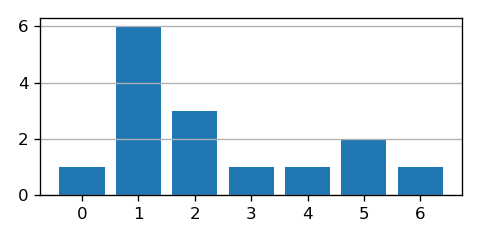
\includegraphics[width=4cm]{Images/histogram1.png} \\
%\visible<2>{\textbf{Output \texttt{data}}
%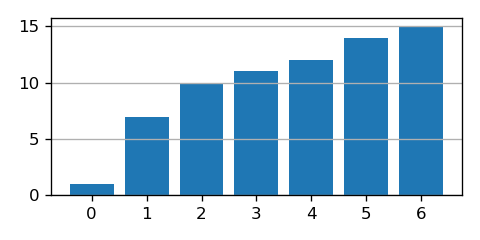
\includegraphics[width=4cm]{Images/histogram1-cum.png}}
%\end{columns}
%\end{frame}


\begin{frame}[fragile]{\texttt{list} slicing}
\begin{python}
data = [1, 6, 3, 1, 1, 2, 1]
\end{python}
\vspace{-5pt}\begin{itemize}\setlength\itemsep{0em}
\item \alert{Indexing:} Accesses an item (\emph{element}) of a \texttt{list} (e.g., ``\pyth{data[2]}'' yields \texttt{3})
\item \alert{Slicing:} Retrieves a \texttt{list} (\emph{subset}) of another \texttt{list}
\vskip1ex
\begin{center}
\resizebox{8cm}{!}{
\begin{tabular}{l|l|c}
    \alert{Syntax} & \alert{Example} & \alert{Slice} \\
    \hline\hline
    \pyth{data[start:end]} & \pyth{data[1:4]} & \pyth{[6, 3, 1]} \\\hline
    \pyth{data[start:]} & \pyth{data[4:]} & \pyth{[1, 2, 1]} \\\hline
    \pyth{data[:end]} & \pyth{data[:3]} & \pyth{[1, 6, 3]} \\\hline
    \pyth{data[start:end:step]} & \pyth{data[2:7:2]} & \pyth{[3, 1, 1]} \\\hline
    \pyth{data[::step]} & \pyth{data[::3]} & \pyth{[1, 1, 1]}
\end{tabular}}
\end{center}
\item Slicing can also be used for \textbf{manipulation} of lists -- \alert{Example:}
\begin{python}
data[2:5] = [-1, -2, -1]
print(data)
\end{python}
\vspace{-5pt}\whitebox{\alert{Output:} \texttt{[1, 6, -1, -2, -1, 2, 1]}}
\end{itemize}
\end{frame}


%\begin{frame}[fragile]{\texttt{list} slicing example}
%\alert{Example}
%\begin{columns}[T,onlytextwidth]
%\column{.65\linewidth}
%\begin{python}
%def fancy_function(data, position):
%    return sum(data[:1 + position])
%
%data = [1, 6, 3, 1, 1, 2, 1]
%for i in range(0, len(data)):
%    print(fancy_function(data, i))
%\end{python}
%\column{.25\linewidth}
%\begin{visibleenv}<2>
%\alert{Output}
%\small
%\begin{verbatim}
%1
%7
%10
%11
%12
%14
%15
%\end{verbatim}
%\end{visibleenv}
%\end{columns}
%\end{frame}


\begin{frame}{Arrays}
    \begin{textblock*}{4cm}(125mm,65mm) % {block width} (coords)
        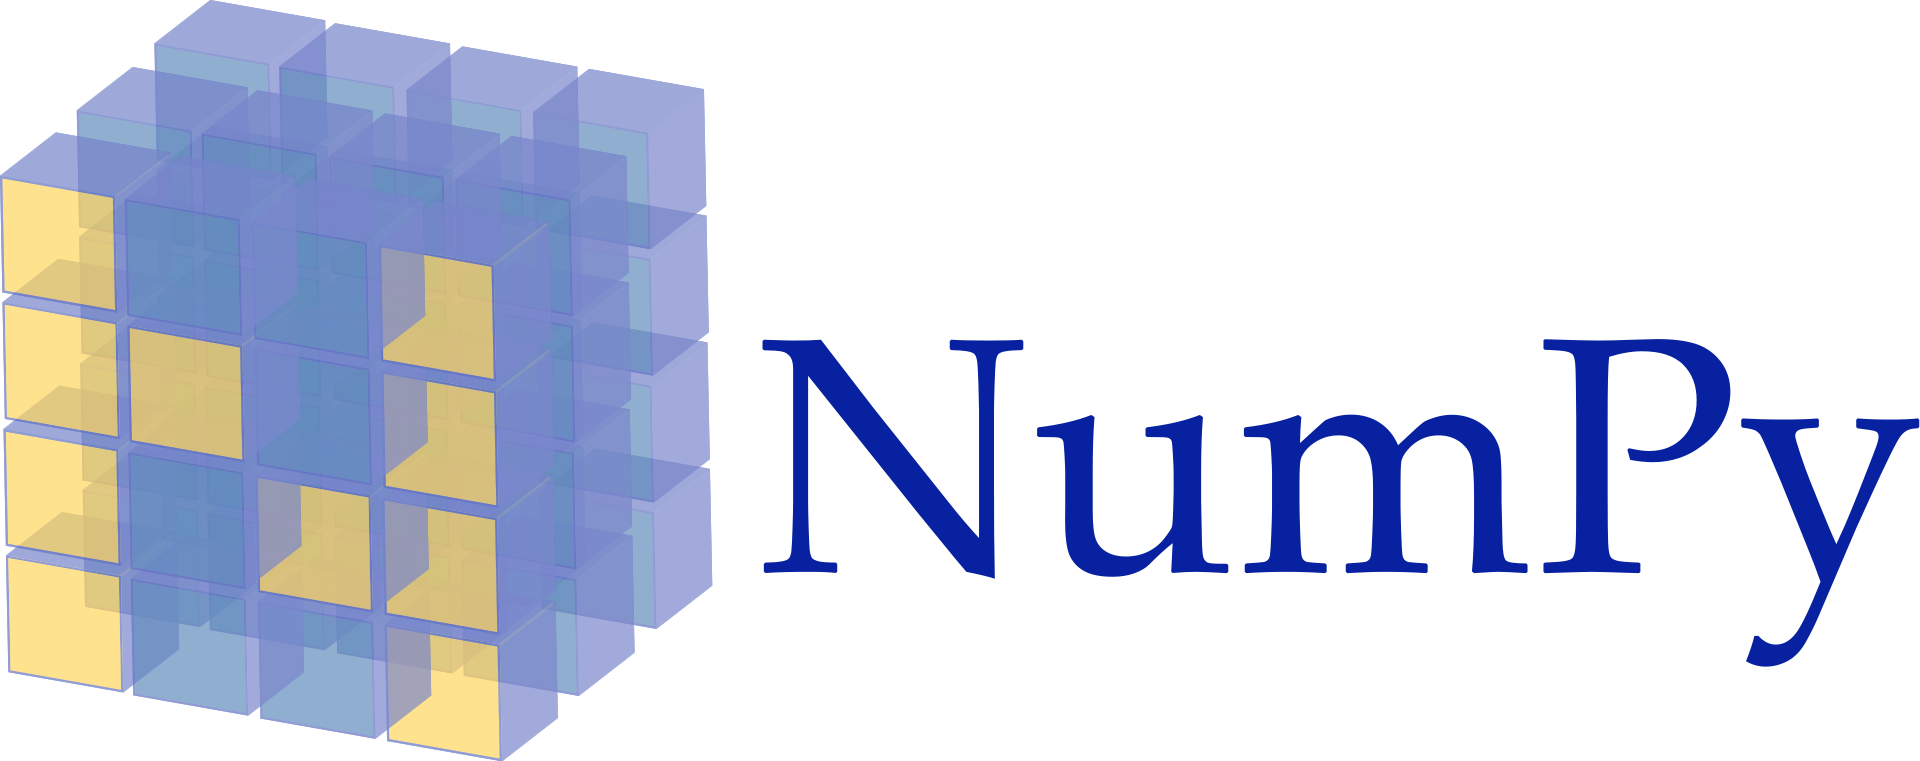
\includegraphics[height=1.8\baselineskip]{Logos/numpy.png}
    \end{textblock*}
    \begin{itemize}
        \item An \alert{array} is a \textbf{list of fixed length and type} (fundamental programming entity in lower-level programming languages, e.g., C, C++, Java, \ldots)
        \vskip2ex
        \item A \alert{multi-dimensional array} is an array with multiple axes
        \begin{itemize}
            \item \textbf{Application examples:} Vector, matrix, 2-D or 3-D image, \ldots
            \item \textbf{In Python:} Represented by objects of the type \texttt{numpy.ndarray} (\texttt{numpy} module)
        \end{itemize}
    \end{itemize}
\end{frame}


\begin{frame}[fragile]{Working with arrays}
\begin{itemize}
\item An \alert{array} is an object of the type \pyth{numpy.ndarray}
\item \textbf{Load the \pyth{numpy} module:}
\begin{python}
import numpy
\end{python}
\item \textbf{Create a new \pyth{float}-type array} filled with zeros:
\begin{minipage}{\linewidth}\vspace{-3pt}
\begin{columns}[onlytextwidth]
\column{.38\linewidth}
\begin{python}
array = numpy.zeros(shape)
\end{python}
\column{.1\linewidth}
\centering or
\column{.47\linewidth}
\begin{python}
array = numpy.zeros(shape, float)
\end{python}
\end{columns}
\end{minipage}
\pyth{shape} is a list which specifies the \textbf{array size} (e.g., ``\pyth{[32, 64]}'' corresponds to a 2-D array with 32 rows and 64 columns)
\item \pyth{array.ndim} evaluates to the \textbf{number of the array dimensions}
\item \pyth{array} is called \alert{flat} if it is single-dimensional (\pyth{array.ndim }\pyth{==}\texttt{ }\pyth{1})
\end{itemize}
\end{frame}


\begin{frame}[fragile]{Arrays and lists}
\textbf{Arrays can also be created from lists}
\vskip2ex
\alert{Example 1:} List of \underline{values}
\begin{columns}[T,onlytextwidth]
\column{.8\linewidth}
\begin{python}
array1 = numpy.asarray([1, 2, 3])
print(array1)
print(f'Dimensions: {array1.ndim}')
\end{python}
\column{.15\linewidth}
\alert{Output}
\begin{verbatim}
[1 2 3]
Dimensions: 1
\end{verbatim}
\end{columns}
\vskip1ex
\alert{Example 2:} List of \underline{rows}
\begin{columns}[T,onlytextwidth]
\column{.8\linewidth}
\begin{python}
array2 = numpy.asarray([[1, 2, 3], [4, 5, 6], [7, 8, 9]])
print(array2)
print(f'Dimensions: {array2.ndim}')
\end{python}
\column{.15\linewidth}
\alert{Output}
\begin{verbatim}
[[1 2 3]
 [4 5 6]
 [7 8 9]]
Dimensions: 2
\end{verbatim}
\end{columns}
\end{frame}


\begin{frame}[fragile]{Array indexing and slicing}
\small\textbf{Arrays can be sliced and indexed \alert{analogously to lists}}
\vskip2ex
\alert{Example 1} -- Indexing
\begin{columns}[T,onlytextwidth]
\column{.8\linewidth}
\begin{python}
array1 = numpy.asarray([[1, 2], [3, 4]])
print(array1[0, 0])
\end{python}
\column{.15\linewidth}
\alert{Output}
\begin{Verbatim}[fontsize=\small]
1
\end{Verbatim}
\end{columns}
\alert{Example 2} -- Slicing
\begin{columns}[T,onlytextwidth]
\column{.8\linewidth}
\begin{python}
array1 = numpy.asarray([[1, 2, 3], [4, 5, 6], [7, 8, 9]])
print(array1[:2, 1:])
\end{python}
\column{.15\linewidth}
\alert{Output}
\begin{Verbatim}[fontsize=\small]
[[2 3]
 [5 6]]
\end{Verbatim}
\end{columns}
\vspace{-0.5mm}
\alert{Example 3} -- Slicing
\begin{columns}[T,onlytextwidth]
\column{.8\linewidth}
\begin{python}
array1 = numpy.zeros([3, 3])
array2 = numpy.asarray([[1, 2], [3, 4]])
array1[1:, :2] = array2
print(array1)
\end{python}
\column{.15\linewidth}
\alert{Output}
\begin{Verbatim}[fontsize=\small]
[[0. 0. 0.]
 [1. 2. 0.]
 [3. 4. 0.]]
\end{Verbatim}
\end{columns}
\end{frame}


\makesectionframe{Understanding errors\\\&\\Common mistakes}

\begin{frame}[fragile]{Tracebacks}
\begin{columns}
\column{\linewidth}
\parbox{\linewidth+2cm}{\begin{itemize}
    \item Python provides a so-called \emph{traceback} when an error occurs
    \item \textbf{Reading a traceback} leads to the error you have made (fundamental programming skill)
\end{itemize}}
\column{0pt}
\end{columns}
\vskip3ex
\begin{columns}[T]
\column{.42\linewidth}
\alert{Example}
\begin{python}
def get_item(data, i):
    return data[i]

print(get_item([1, 6, 3], 3))
\end{python}
\tikz\node[coordinate,yshift=1cm,xshift=45mm] (n1) {};
\vskip1ex
\begin{visibleenv}<3>
\begin{commonmistake}{\linewidth}
\textbf{\texttt{IndexError}:} Accessing list/array items out of range
\end{commonmistake}\end{visibleenv}
\column{.55\linewidth}
\begin{visibleenv}<2->
\alert{Output}
\begin{lstlisting}
-----------------------------------------------------------
IndexError                Traceback (most recent call last)
<ipython-input-20-bf91d868e666> in <module>
      2     return data[i]
      3 
|\tikz[na]\node[coordinate,xshift=-3mm] (n2) {};|----> 4 print(get_item([1, 6, 3], 3))

<ipython-input-20-bf91d868e666> in get_item(data, i)
      1 def get_item(data, i):
|\tikz[na]\node[coordinate,xshift=-3mm] (n3) {};|----> 2     return data[i]
      3 
      4 print(get_item([1, 6, 3], 3))

|\hiliteon<3>{IndexError}|: list index out of range
\end{lstlisting}
\end{visibleenv}
\end{columns}
\begin{tikzpicture}[overlay]
    \path[->,ultra thick,color=red,shorten >=3pt]<3> (n2) edge [bend right] (n1);
    \path[->,ultra thick,color=red,shorten >=3pt]<3> (n3) edge [bend left] (n2);
\end{tikzpicture}
\end{frame}


\begin{frame}[fragile]{Common mistakes}
\begin{columns}[T]
\column{.42\linewidth}
\alert{Example}
\begin{python}
def reverse(string):
    result = ''
    for character in string:
    result = character + result
    return result

reverse('Hello World')
\end{python}
\tikz\node[coordinate,yshift=25mm,xshift=45mm] (n1) {};
\column{.55\linewidth}
\begin{visibleenv}<2->
\alert{Output}
\begin{lstlisting}
  File "<ipython-input-21-e6c02796aba8>", line 4
    |\tikz[na]\node[coordinate,xshift=-2mm] (n2) {};|result = character + result
         ^
|\hiliteon<3>{IndentationError}|: expected an indented block
\end{lstlisting}
\end{visibleenv}
\vskip3ex
\begin{visibleenv}<3>
\begin{commonmistake}{\linewidth}
\textbf{\texttt{IndentationError}:} Wrong indentation
\end{commonmistake}\end{visibleenv}
\end{columns}
\begin{tikzpicture}[overlay]
    \path[->,ultra thick,color=red]<3> (n2) edge [bend right] (n1);
\end{tikzpicture}
\end{frame}


\begin{frame}[fragile]{Common mistakes}
\begin{columns}[T]
\column{.42\linewidth}
\alert{Example}
\begin{python}
data = [1, 6, 3, 1, 1, 2, 1]
for i in range(0, len(data)):
    print(fancy_function(data, i))

def fancy_function(data, position):
    return sum(data[:1 + position])
\end{python}
\tikz\node[coordinate,yshift=22mm,xshift=52mm] (n1) {};
\column{.55\linewidth}
\begin{visibleenv}<2->
\alert{Output}
\begin{lstlisting}
-----------------------------------------------------------------
NameError                       Traceback (most recent call last)
<ipython-input-24-fcf3bd0f1bea> in <module>
      1 data = [1, 6, 3, 1, 1, 2, 1]
      2 for i in range(0, len(data)):
|\tikz[na]\node[coordinate,yshift=1mm] (n2) {};|----> 3     print(fancy_function(data, i))
      4 
      5 def fancy_function(data, position):

|\hiliteon<3>{NameError}|: name 'fancy_function' is not defined
\end{lstlisting}
\end{visibleenv}
\vskip3ex
\begin{visibleenv}<3>
\begin{commonmistake}{\linewidth}
\textbf{\texttt{NameError}:} Function used before definition
\end{commonmistake}\end{visibleenv}
\end{columns}
\begin{tikzpicture}[overlay]
    \path[->,ultra thick,color=red]<3> (n2) edge [bend right] (n1);
\end{tikzpicture}
\end{frame}


\begin{frame}[fragile]{Common mistakes}
\begin{columns}[T]
\column{.42\linewidth}
\alert{Example}
\begin{python}
for character in 'Hello World':
    result = character + result
print(result)
\end{python}
\tikz\node[coordinate,yshift=14mm,xshift=48mm] (n1) {};
\column{.55\linewidth}
\begin{visibleenv}<2->
\alert{Output}
\begin{lstlisting}
-----------------------------------------------------------------
NameError                       Traceback (most recent call last)
<ipython-input-26-bc66d091382b> in <module>
      1 for character in 'Hello World':
|\tikz[na]\node[coordinate,yshift=1mm] (n2) {};|----> 2     result = character + result
      3 print(result)

|\hiliteon<3>{NameError}|: name 'result' is not defined
\end{lstlisting}
\end{visibleenv}
\vskip3ex
\begin{visibleenv}<3>
\begin{commonmistake}{\linewidth}
\textbf{\texttt{NameError}:} Variable usage before assignment
\end{commonmistake}\end{visibleenv}
\end{columns}
\begin{tikzpicture}[overlay]
    \path[->,ultra thick,color=red]<3> (n2) edge [bend right] (n1);
\end{tikzpicture}
\end{frame}


\begin{frame}[fragile]{Common mistakes}
\begin{columns}[T]
\column{.42\linewidth}
\alert{Example 1}
\begin{python}
data = [3, 1, 6, 11, 5, 2, 1]
for i in range(0, len(data) / 2):
    print(data[i])
\end{python}
\tikz\node[coordinate,yshift=12mm,xshift=43mm] (n1) {};
\vskip2ex
\begin{visibleenv}<4>
\alert{Example 2}
\begin{python}
data = [3, 1, 6, 11, 5, 2, 1]
for i in range(0, len(data)):
    print(data[i / 2])
\end{python}
\tikz\node[coordinate,yshift=8mm,xshift=27mm] (n3) {};
\tikz\node[coordinate,yshift=-3mm,xshift=32mm] (n4) {};
\end{visibleenv}
\column{.55\linewidth}
\begin{visibleenv}<2->
\alert{Output}
\begin{lstlisting}
-----------------------------------------------------------------
TypeError                       Traceback (most recent call last)
<ipython-input-27-af826dd5c45c> in <module>
      1 data = [3, 1, 6, 11, 5, 2, 1]
|\tikz[na]\node[coordinate,xshift=-1mm] (n2) {};|----> 2 for i in range(0, len(data) / 2):
      3     print(data[i])
      4 

|\hiliteon<3->{TypeError}|: 'float' object cannot be interpreted as an integer
\end{lstlisting}
\end{visibleenv}
\vskip3ex
\begin{visibleenv}<3->
\begin{commonmistake}{\linewidth}
\textbf{\texttt{TypeError}:} The object used for \texttt{range}, indexing, or slicing is not of type \texttt{int}
\end{commonmistake}\end{visibleenv}
\end{columns}
\begin{tikzpicture}[overlay]
    \path[->,ultra thick,color=red]<3-> (n2) edge [bend left] (n1);
    \path[->,ultra thick,color=red]<4-> (n4) edge [] (n3);
\end{tikzpicture}
\end{frame}


\makesectionframe{Questions?}

\end{document}
